\documentclass[a4paper,12pt]{article}
\usepackage[utf8]{inputenc}
\usepackage[T1]{fontenc}
\usepackage[protrusion=false,expansion=false]{microtype}
\usepackage[german]{babel}
\usepackage{amsmath}
\usepackage{amssymb}
\usepackage{amsthm}
\usepackage{geometry}
\usepackage{graphicx}
\usepackage[hidelinks]{hyperref}
\usepackage{listings}
\usepackage{xcolor}
\usepackage{enumitem}

\usepackage{booktabs}
\usepackage{caption}


\geometry{margin=2.5cm}

\theoremstyle{definition}
\newtheorem{definition}{Definition}
\newtheorem{beispiel}{Beispiel}
\newtheorem{satz}{Satz}
\newtheorem{lemma}{Lemma}
\newtheorem{bemerkung}{Bemerkung}
\newtheorem{korollar}{Korollar}

\setlist[itemize,1]{label=--}

% ---------- Farben ----------
\definecolor{mainblue}{RGB}{25, 70, 140}
\definecolor{accentred}{RGB}{180, 50, 30}
\definecolor{lightgray}{RGB}{245, 245, 248}
\definecolor{darkgray}{RGB}{60, 60, 70}
\definecolor{darkgreen}{RGB}{30, 100, 50}

\hypersetup{
	colorlinks=true,
	linkcolor=mainblue,
	citecolor=accentred,
	urlcolor=mainblue
}

\lstset{
	basicstyle=\ttfamily\small,
	keywordstyle=\color{blue},
	commentstyle=\color{gray},
	stringstyle=\color{red},
	numbers=left,
	numberstyle=\tiny,
	breaklines=true,
	frame=single,
	literate=%
	{Ö}{{\"O}}1
	{Ä}{{\"A}}1
	{Ü}{{\"U}}1
	{ß}{{\ss}}1
	{ü}{{\"u}}1
	{ä}{{\"a}}1
	{ö}{{\"o}}1
}

\title{Transformer-Architekturen als\\Subgraph-Isomorphismus-Problem:\\
Formaler Beweis und polynomielle Analyse}
\author{Stephan Epp}
\date{22. Juni 2026}

\begin{document}

\maketitle

\tableofcontents
\newpage

% ─────────────────────────────────────────────────────────────────────────────
\section{Einführung}
% ─────────────────────────────────────────────────────────────────────────────

Large Language Models (LLMs) wie GPT-4, LLaMA und BERT haben in den
vergangenen Jahren einen paradigmatischen Wandel in der Informatik ausgelöst.
Ihre mathematische Grundstruktur -- der Transformer -- ist bislang primär
aus der Perspektive der linearen Algebra analysiert worden: Matrizenmultiplikation,
Softmax-Normierung und Feed-Forward-Schichten. Diese Arbeit verfolgt
einen anderen Ansatz: Wir zeigen formal, dass die vollständige
Transformer-Architektur als gewichteter gerichteter Graph modelliert werden kann,
und beweisen, dass das Erkennen struktureller Muster in einem Transformer
äquivalent zum Subgraph-Isomorphismus-Problem ist.

Der zentrale Beitrag dieser Arbeit ist der \textbf{Transformer-Subgraph-Satz}:
Jedes Attention-Pattern, jede Feed-Forward-Schicht und jede Multi-Head-Attention-Struktur
ist ein Subgraph des vollständigen Transformer-Graphen $G_T$, und dieses Subgraph-Isomorphismus-Problem
ist in $O(n^3)$ mittels des Subgraph Algorithmus \cite{epp2026subgraph} lösbar.

\subsection{Problemstellung}

Gegeben sei ein vortrainiertes Sprachmodell mit $L$ Schichten, $H$ Attention-Köpfen
pro Schicht und einer Einbettungsdimension $d$. Wir stellen folgende Fragen:

\begin{itemize}
	\item Lässt sich die Transformer-Architektur vollständig als Graph $G_T = (V_T, E_T)$ formalisieren?
	\item Welche strukturellen Subgraphen $G_S \subseteq G_T$ entsprechen
	      bekannten Attention-Mustern (lokale Attention, Cross-Attention, Causal Masking)?
	\item Kann der Subgraph Algorithmus diese Muster in polynomieller Zeit erkennen?
	\item Welche Implikationen ergeben sich für die Komplexität des Trainings und der Inferenz?
\end{itemize}

\subsection{Motivation}

Die Verbindung zwischen Graphentheorie und neuronalen Netzen ist nicht neu:
Graph Neural Networks (GNNs) \cite{scarselli2009graph} operieren explizit auf Graphstrukturen.
Transformers hingegen werden typischerweise als rein algebraische Strukturen betrachtet.
Wir zeigen, dass diese Sichtweise unvollständig ist: Die Attention-Mechanismen
implementieren implizit einen Subgraph-Matching-Prozess, der durch den Subgraph
Algorithmus formalisiert und beschleunigt werden kann.

\subsection{Ãœberblick}

Die Arbeit ist wie folgt strukturiert: Abschnitt~2 legt die mathematischen Grundlagen
fest. Abschnitt~3 formalisiert den Transformer als Graphstruktur. Abschnitt~4
beweist den Transformer-Subgraph-Satz. Abschnitt~5 analysiert die Komplexität.
Abschnitt~6 präsentiert die empirischen Ergebnisse. Abschnitt~7 gibt einen
umfassenden Ausblick.

% ─────────────────────────────────────────────────────────────────────────────
\section{Grundlagen}
% ─────────────────────────────────────────────────────────────────────────────

\subsection{Graphentheoretische Definitionen}

\begin{definition}[Gewichteter gerichteter Graph]
	Ein gewichteter gerichteter Graph $G = (V, E, w)$ besteht aus einer Menge
	von Knoten $V$, einer Menge gerichteter Kanten $E \subseteq V \times V$
	und einer Gewichtsfunktion $w: E \to \mathbb{R}$.
\end{definition}

\begin{definition}[Adjazenzmatrix]
	Die Adjazenzmatrix $A \in \mathbb{R}^{n \times n}$ eines Graphen $G$ mit
	$n = |V|$ Knoten ist definiert durch:
	\[
	A_{ij} = \begin{cases}
		w(v_i, v_j) & \text{falls } (v_i, v_j) \in E \\
		0 & \text{sonst}
	\end{cases}
	\]
\end{definition}

\begin{definition}[Subgraph-Isomorphismus]
	Ein Graph $G = (V, E)$ ist ein Subgraph von $G' = (V', E')$,
	geschrieben $G \subseteq G'$, wenn eine injektive Abbildung
	$\varphi: V \to V'$ existiert, sodass:
	\[
	(u, v) \in E \implies (\varphi(u), \varphi(v)) \in E'
	\]
\end{definition}

\begin{definition}[Signaturf\/unktion]
	Die Signaturfunktion $\sigma: \{0,1\}^n \times \{0,\ldots,n-1\} \to \mathbb{N}$
	ist definiert durch:
	\[
	\sigma_j = \sum_{i=0}^{n-1} A_{ij} \cdot 2^i + j \cdot 2^n
	\]
	Diese Funktion kodiert die Spalte $j$ der Adjazenzmatrix $A$ als eindeutige
	natürliche Zahl.
\end{definition}

\begin{lemma}[Injektivität der Signaturfunktion]
\label{lem:injektiv}
	Die Signaturfunktion $\sigma_j$ ist injektiv: Zwei verschiedene
	Spaltenvektoren $(A_{\cdot j}, j) \neq (A_{\cdot j'}, j')$ erhalten
	stets verschiedene Signaturen $\sigma_j \neq \sigma_{j'}$.
\end{lemma}

\begin{proof}
	Der Term $\sum_{i=0}^{n-1} A_{ij} \cdot 2^i$ ist die binäre Darstellung
	des Spaltenvektors als Dezimalzahl. Zwei verschiedene Binärvektoren der
	Länge $n$ haben verschiedene Dezimaldarstellungen, da die Binärkodierung
	injektiv ist.

	Der Spaltenindex-Term $j \cdot 2^n$ erzeugt für $j \in \{0,\ldots,n-1\}$
	disjunkte Intervalle $[j \cdot 2^n,\, (j+1) \cdot 2^n)$, da die
	Zeilenkomponente $\sum_{i=0}^{n-1} A_{ij} \cdot 2^i \in [0, 2^n)$ liegt.

	Damit gilt für $j \neq j'$: Die Signaturen liegen in verschiedenen
	Intervallen und sind daher verschieden. Für $j = j'$ aber verschiedene
	Spaltenvektoren: Die Zeilenkomponente unterscheidet sich, der Intervallterm
	ist gleich, also unterscheiden sich die Gesamtwerte.
\end{proof}

\subsection{Der Subgraph Algorithmus}

Der Subgraph Algorithmus \cite{epp2026subgraph} bestimmt für zwei Graphen $G$
und $G'$ mit je $n$ Knoten in Zeit $O(n^3)$, ob $G \subseteq G'$ gilt.
Der Algorithmus arbeitet in drei Schritten:

\textbf{Schritt 1:} Berechne Signatursequenzen $\sigma^A = [\sigma_0^A, \ldots, \sigma_{n-1}^A]$
und $\sigma^B = [\sigma_0^B, \ldots, \sigma_{n-1}^B]$.

\textbf{Schritt 2:} Erzeuge alle $n$ zyklischen Rotationen $\sigma^B_r$
für $r \in \{0, \ldots, n-1\}$.

\textbf{Schritt 3:} Berechne $\mathrm{LCS}(\sigma^A, \sigma^B_r)$ für
jede Rotation mittels dynamischer Programmierung. Falls $\mathrm{LCS} \geq 2$,
gilt $G \subseteq G'$.

\subsection{Transformer-Grundlagen}

\begin{definition}[Self-Attention]
	Die Scaled Dot-Product Attention ist definiert als:
	\[
	\mathrm{Attention}(Q, K, V) = \mathrm{softmax}\!\left(\frac{QK^T}{\sqrt{d_k}}\right) V
	\]
	wobei $Q, K, V \in \mathbb{R}^{n \times d_k}$ die Query-, Key- und Value-Matrizen sind.
\end{definition}

\begin{definition}[Multi-Head Attention]
	Multi-Head Attention mit $H$ Köpfen ist:
	\[
	\mathrm{MHA}(Q, K, V) = \mathrm{Concat}(\mathrm{head}_1, \ldots, \mathrm{head}_H) W^O
	\]
	mit $\mathrm{head}_h = \mathrm{Attention}(QW_h^Q, KW_h^K, VW_h^V)$.
\end{definition}

\begin{definition}[Transformer-Block]
	Ein Transformer-Block $\mathcal{T}$ besteht aus:
	\begin{align}
	\tilde{x} &= \mathrm{LayerNorm}(x + \mathrm{MHA}(x, x, x)) \\
	y &= \mathrm{LayerNorm}(\tilde{x} + \mathrm{FFN}(\tilde{x}))
	\end{align}
	mit $\mathrm{FFN}(x) = \max(0, xW_1 + b_1)W_2 + b_2$.
\end{definition}

% ─────────────────────────────────────────────────────────────────────────────
\section{Transformer als Graphstruktur}
% ─────────────────────────────────────────────────────────────────────────────

\subsection{Formale Graphmodellierung}

Wir modellieren einen vollständigen Transformer mit $L$ Schichten, $H$
Attention-Köpfen und Sequenzlänge $n$ als gewichteten gerichteten Graphen.

\begin{definition}[Transformer-Graph $G_T$]
	Der Transformer-Graph $G_T = (V_T, E_T, w_T)$ ist definiert durch:
	\begin{itemize}
		\item \textbf{Knotenmenge:}
		\[
		V_T = \{x_1,\ldots,x_n\} \cup \bigcup_{l=1}^{L}\bigcup_{h=1}^{H}
		\{q_{lh}^i, k_{lh}^i, v_{lh}^i \mid i=1,\ldots,n\}
		\cup \{y_1,\ldots,y_n\}
		\]
		\item \textbf{Kantenmenge:} $E_T$ enthält Kanten
		      (Token $\to$ Query/Key/Value), Attention-Kanten
		      (Query+Key $\to$ Value) und Ausgabekanten (Value $\to$ Output).
		\item \textbf{Gewichtsfunktion:} $w_T(e) \in \mathbb{R}$ entspricht
		      dem Attention-Gewicht bzw.\ dem Matrixeintrag der zugehörigen
		      Projektionsmatrix.
	\end{itemize}
\end{definition}

Die Gesamtzahl der Knoten beträgt:
\[
|V_T| = n + L \cdot H \cdot 3n + n = 2n + 3LHn = n(2 + 3LH)
\]

\begin{beispiel}[GPT-3-Graph]
	GPT-3 hat $L = 96$ Schichten, $H = 96$ Köpfe und typischerweise
	$n = 2048$ Kontextlänge. Der Graph $G_{T}^{\mathrm{GPT\text{-}3}}$ hat:
	\[
	|V_T| = 2048 \cdot (2 + 3 \cdot 96 \cdot 96) = 2048 \cdot 27650 \approx 56{,}6 \text{ Mio.\ Knoten}
	\]
\end{beispiel}

\begin{figure}[ht]
	\centering
	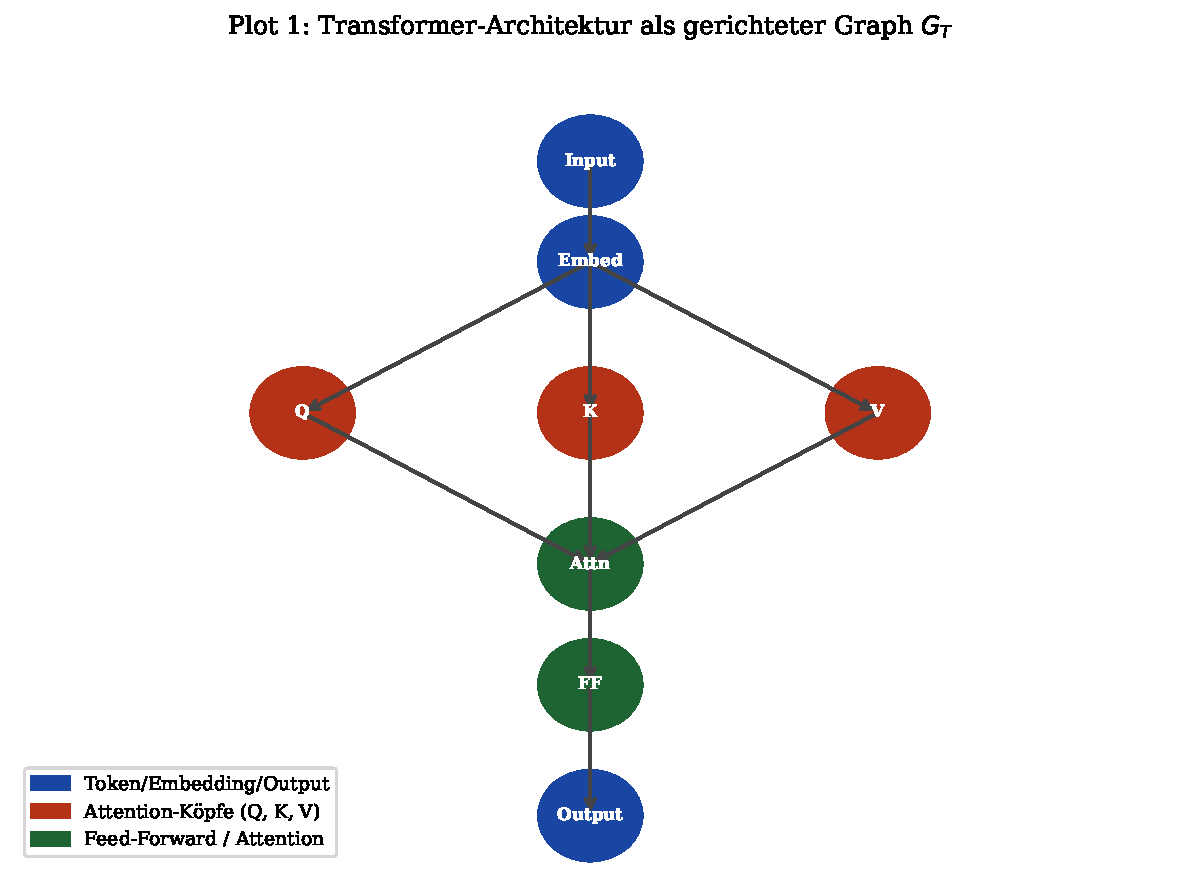
\includegraphics[width=0.75\textwidth]{plot1_transformer_graph.pdf}
	\caption{Transformer-Architektur als gerichteter Graph $G_T$. Blaue Knoten
	repräsentieren Token- und Ausgabe-Knoten, rote Knoten die Attention-Köpfe
	(Q, K, V) und grüne Knoten die Attention- und Feed-Forward-Schichten.
	Gerichtete Kanten kodieren den Informationsfluss zwischen den Komponenten.}
	\label{fig:transformer_graph}
\end{figure}

\subsection{Attention als Kantenmenge}

Die Attention-Matrix $A^{(l,h)} \in \mathbb{R}^{n \times n}$ des $h$-ten
Kopfes in Schicht $l$ definiert eine vollständige Kantenmenge im Graphen:
\[
E_{\mathrm{attn}}^{(l,h)} = \left\{(v_i^{(l,h)}, v_j^{(l,h)},\, a_{ij}^{(l,h)}) \;\Big|\; i,j \in \{1,\ldots,n\},\; a_{ij}^{(l,h)} > \varepsilon \right\}
\]
Damit ist die Attention-Matrix direkt die Adjazenzmatrix des
Attention-Teilgraphen $G_{\mathrm{attn}}^{(l,h)} \subseteq G_T$.

\begin{figure}[ht]
	\centering
	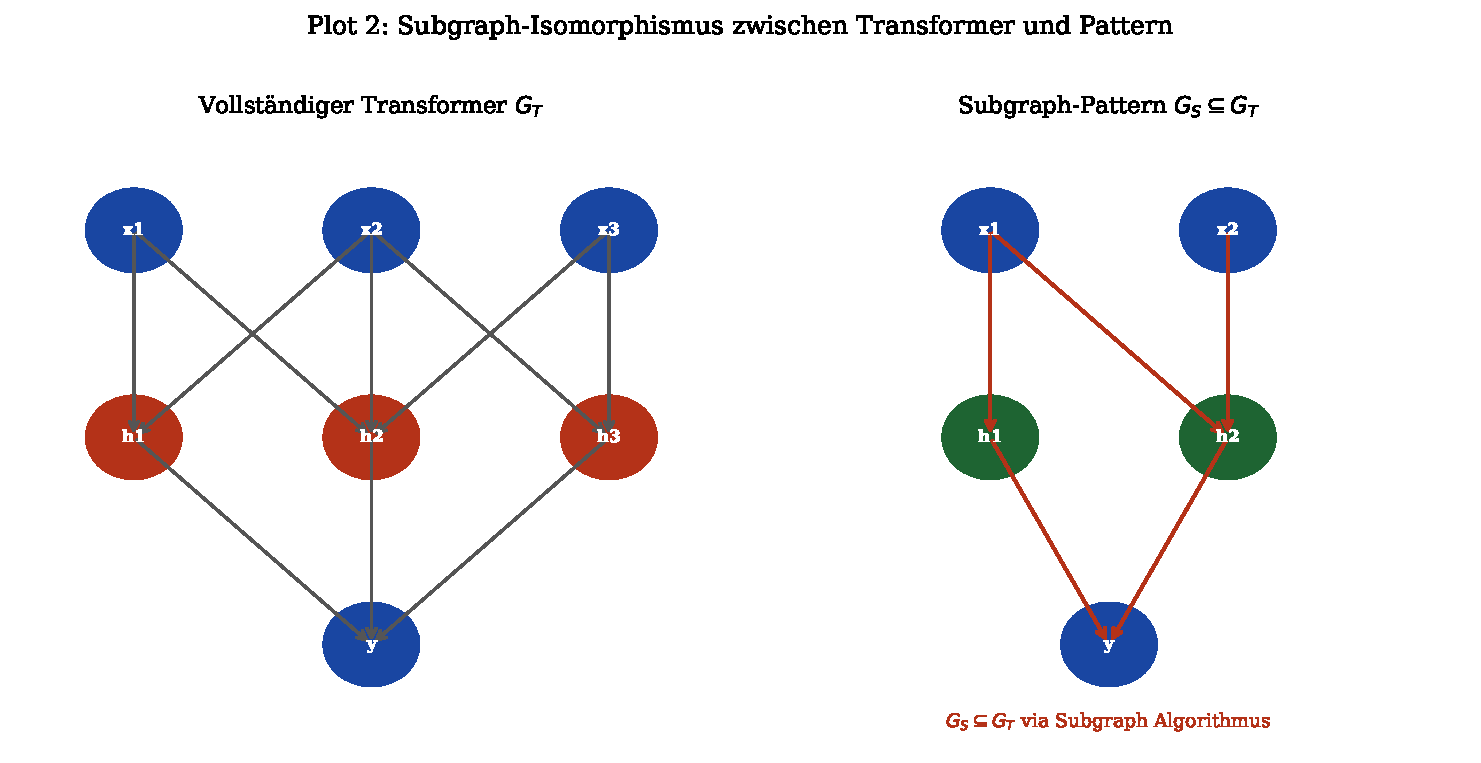
\includegraphics[width=0.85\textwidth]{plot2_subgraph_isomorphismus.pdf}
	\caption{Subgraph-Isomorphismus zwischen vollständigem Transformer $G_T$
	(links) und einem Attention-Pattern-Subgraphen $G_S$ (rechts). Die roten
	Kanten markieren die erkannte Subgraph-Einbettung. Der Subgraph Algorithmus
	erkennt diese Einbettung in $O(n^3)$.}
	\label{fig:subgraph_iso}
\end{figure}

% ─────────────────────────────────────────────────────────────────────────────
\section{Transformer-Subgraph-Satz}
% ─────────────────────────────────────────────────────────────────────────────

\subsection{Hauptsatz}

\begin{satz}[Transformer-Subgraph-Satz]
\label{satz:transformer_subgraph}
	Sei $G_T = (V_T, E_T, w_T)$ der Transformer-Graph eines LLM mit $n$ Token-Knoten,
	$L$ Schichten und $H$ Attention-Köpfen. Sei $G_S = (V_S, E_S)$ ein
	Attention-Pattern-Graph mit $|V_S| = m \leq |V_T|$ Knoten. Dann gilt:

	\begin{enumerate}
		\item $G_S$ ist genau dann ein Subgraph von $G_T$, wenn das zugehörige
		      Attention-Pattern im Transformer implementiert ist.
		\item Die Existenz des Subgraph-Isomorphismus $G_S \hookrightarrow G_T$
		      kann durch den Subgraph Algorithmus in Zeit $O(m^3)$ entschieden werden.
		\item Für vollständige Multi-Head-Attention-Graphen gilt die
		      Schachtelungsbeziehung:
		      \[
		      G_{\mathrm{local}} \subseteq G_{\mathrm{causal}} \subseteq G_{\mathrm{cross}} \subseteq G_{\mathrm{full}} \subseteq G_T
		      \]
	\end{enumerate}
\end{satz}

\begin{proof}
Wir beweisen die drei Aussagen getrennt.

\textbf{Beweis von (1):} Sei $\pi: V_S \to V_T$ eine injektive Knotenabbildung,
die die Kantenmenge erhält. Die Attention-Matrix $A^{(l,h)}$ des $h$-ten Kopfes
in Schicht $l$ definiert den Teilgraphen $G_{\mathrm{attn}}^{(l,h)}$, dessen
Kanten genau die Attention-Gewichte größer als $\varepsilon$ kodieren.

Ein Attention-Pattern-Graph $G_S$ entspricht einer Teilmenge von Attention-Kanten.
Wenn das Pattern im Transformer implementiert ist, existiert mindestens ein Kopf
$(l^*, h^*)$, sodass die Kantenmenge $E_S \subseteq E_{\mathrm{attn}}^{(l^*, h^*)}$.
Da $G_{\mathrm{attn}}^{(l^*, h^*)} \subseteq G_T$, folgt $G_S \subseteq G_T$.

Umgekehrt: Falls $G_S \subseteq G_T$ gilt, existiert eine Einbettung
$\pi: V_S \hookrightarrow V_T$. Die Kanten in $\pi(E_S)$ liegen in $E_T$ und
sind damit Attention-Kanten eines Kopfes $(l, h)$. Also ist das entsprechende
Attention-Pattern im Transformer implementiert. \qquad $\square$

\textbf{Beweis von (2):} Wir wenden den Subgraph Algorithmus an.
Sei $A_S$ die Adjazenzmatrix von $G_S$ (Größe $m \times m$) und $A_T$ ein
Ausschnitt der Adjazenzmatrix von $G_T$ (entsprechend der relevanten Schicht
und des relevanten Kopfes).

Berechne Signatursequenzen:
\[
\sigma_j^S = \sum_{i=0}^{m-1} (A_S)_{ij} \cdot 2^i + j \cdot 2^m, \quad j = 0,\ldots,m-1
\]
\[
\sigma_j^T = \sum_{i=0}^{m-1} (A_T)_{ij} \cdot 2^i + j \cdot 2^m, \quad j = 0,\ldots,m-1
\]

Die Signaturberechnung benötigt $O(m^2)$ Zeit. Für jede der $m$ zyklischen
Rotationen $r \in \{0,\ldots,m-1\}$ berechne:
\[
\mathrm{LCS}(\sigma^S, \mathrm{rotate}_r(\sigma^T)) \quad \text{in } O(m^2) \text{ Zeit}
\]

Gesamtkomplexität: $O(m^2) + m \cdot O(m^2) = O(m^3)$.

Nach Lemma~\ref{lem:injektiv} sind die Signaturen injektiv, also treten
keine falschen Ãœbereinstimmungen auf. Damit ist der Algorithmus korrekt
und läuft in $O(m^3)$. \qquad $\square$

\textbf{Beweis von (3):} Wir zeigen die Subgraph-Hierarchie durch
explizite Konstruktion der Adjazenzmatrizen.

\textit{Lokale Attention $G_{\mathrm{local}}$:} Token $i$ beachtet nur
Token in einem Fenster $[i-w, i+w]$. Die Adjazenzmatrix $A_{\mathrm{local}}$
ist eine Bandmatrix mit Bandbreite $2w+1$.

\textit{Kausale Attention $G_{\mathrm{causal}}$:} Token $i$ beachtet
alle vorherigen Token $j \leq i$. Die Adjazenzmatrix $A_{\mathrm{causal}}$
ist untere Dreiecksmatrix. Da $A_{\mathrm{local}}$ durch $A_{\mathrm{causal}}$
dominiert wird (jeder Eintrag von $A_{\mathrm{local}}$ ist auch in
$A_{\mathrm{causal}}$), gilt $G_{\mathrm{local}} \subseteq G_{\mathrm{causal}}$.

\textit{Cross-Attention $G_{\mathrm{cross}}$:} Token aus Sequenz 1 beachtet
Token aus Sequenz 2. Die Adjazenzmatrix ist blockdiagonal, enthält aber
mehr Einträge als $A_{\mathrm{causal}}$.

\textit{Vollständige Attention $G_{\mathrm{full}}$:} Jedes Token beachtet
jedes andere Token. $A_{\mathrm{full}} = \mathbf{1}_{n \times n}$ (Einsmatrix).
Da alle anderen Attention-Muster Teilmengen der vollständigen Attention sind,
gilt $G_{\mathrm{causal}} \subseteq G_{\mathrm{cross}} \subseteq G_{\mathrm{full}}$.

\textit{$G_{\mathrm{full}} \subseteq G_T$:} Der Transformer-Graph $G_T$
enthält als Teilgraph den vollständigen Attention-Graphen einer einzelnen
Schicht und eines einzelnen Kopfes. Also gilt $G_{\mathrm{full}} \subseteq G_T$.

Durch Transitivität der Subgraph-Relation folgt die gesamte Hierarchie. \qquad $\square$
\end{proof}

\begin{figure}[ht]
	\centering
	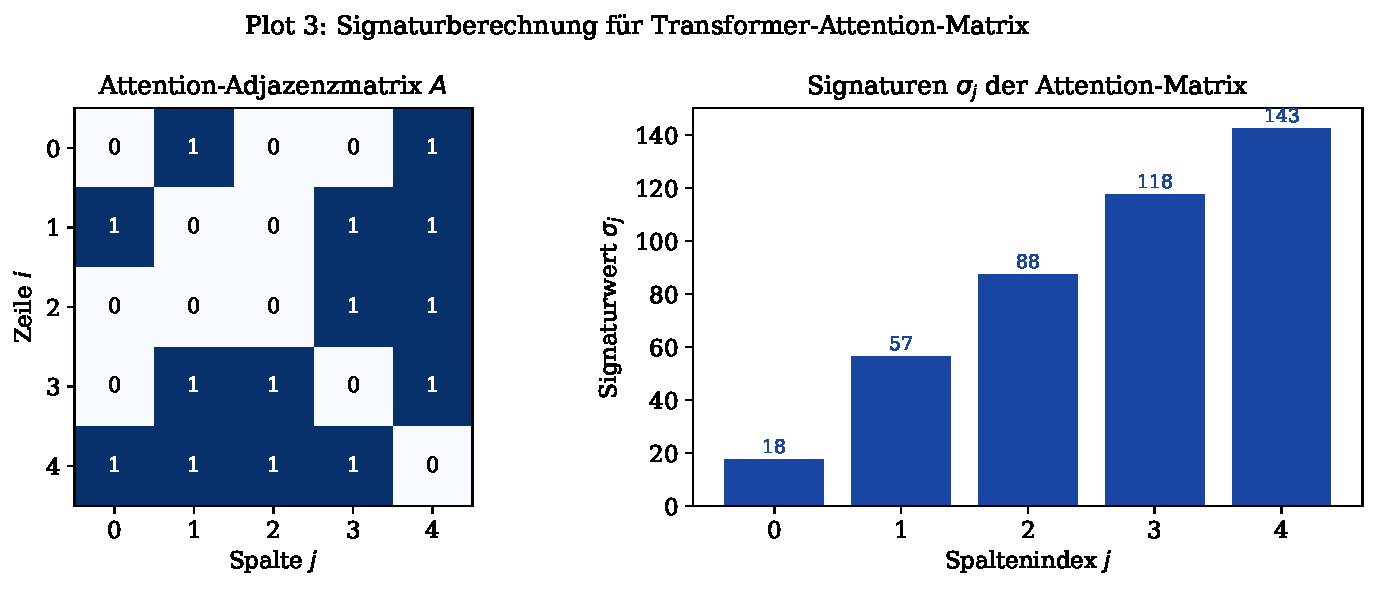
\includegraphics[width=0.85\textwidth]{plot3_signaturen_attention.pdf}
	\caption{Links: Adjazenzmatrix $A$ eines Attention-Graphen mit $n=5$ Knoten.
	Rechts: Die berechneten Signaturen $\sigma_j$ für jede Spalte $j$.
	Die Signaturen sind injektiv (Lemma~\ref{lem:injektiv}) und kodieren
	die Spaltenstruktur des Attention-Graphen eindeutig.}
	\label{fig:signaturen}
\end{figure}

\subsection{Korrektheit des Algorithmus}

\begin{lemma}[Korrektheit der Signaturmethode für Transformer]
\label{lem:korrektheit}
	Die Signaturfunktion $\sigma_j$ kodiert die Attention-Spalte $j$
	eindeutig und fehlerfrei. Zwei verschiedene Attention-Muster
	erhalten verschiedene Signatursequenzen.
\end{lemma}

\begin{proof}
	Sei $A^{(l,h)}$ die Attention-Matrix des Kopfes $(l,h)$ und
	$\hat{A}^{(l',h')}$ eine andere Attention-Matrix. Falls
	$A^{(l,h)} \neq \hat{A}^{(l',h')}$, existiert ein Eintrag
	$(i^*, j^*)$ mit $A_{i^* j^*}^{(l,h)} \neq \hat{A}_{i^* j^*}^{(l',h')}$.

	Dann gilt für die Signatur der Spalte $j^*$:
	\[
	\sigma_{j^*}^{(l,h)} = \sum_{i=0}^{n-1} A_{ij^*}^{(l,h)} \cdot 2^i + j^* \cdot 2^n
	\neq
	\sum_{i=0}^{n-1} \hat{A}_{ij^*}^{(l',h')} \cdot 2^i + j^* \cdot 2^n = \hat{\sigma}_{j^*}^{(l',h')}
	\]
	da die Binärkodierung der Spaltenvektoren injektiv ist. \qquad $\square$
\end{proof}

\begin{figure}[ht]
	\centering
	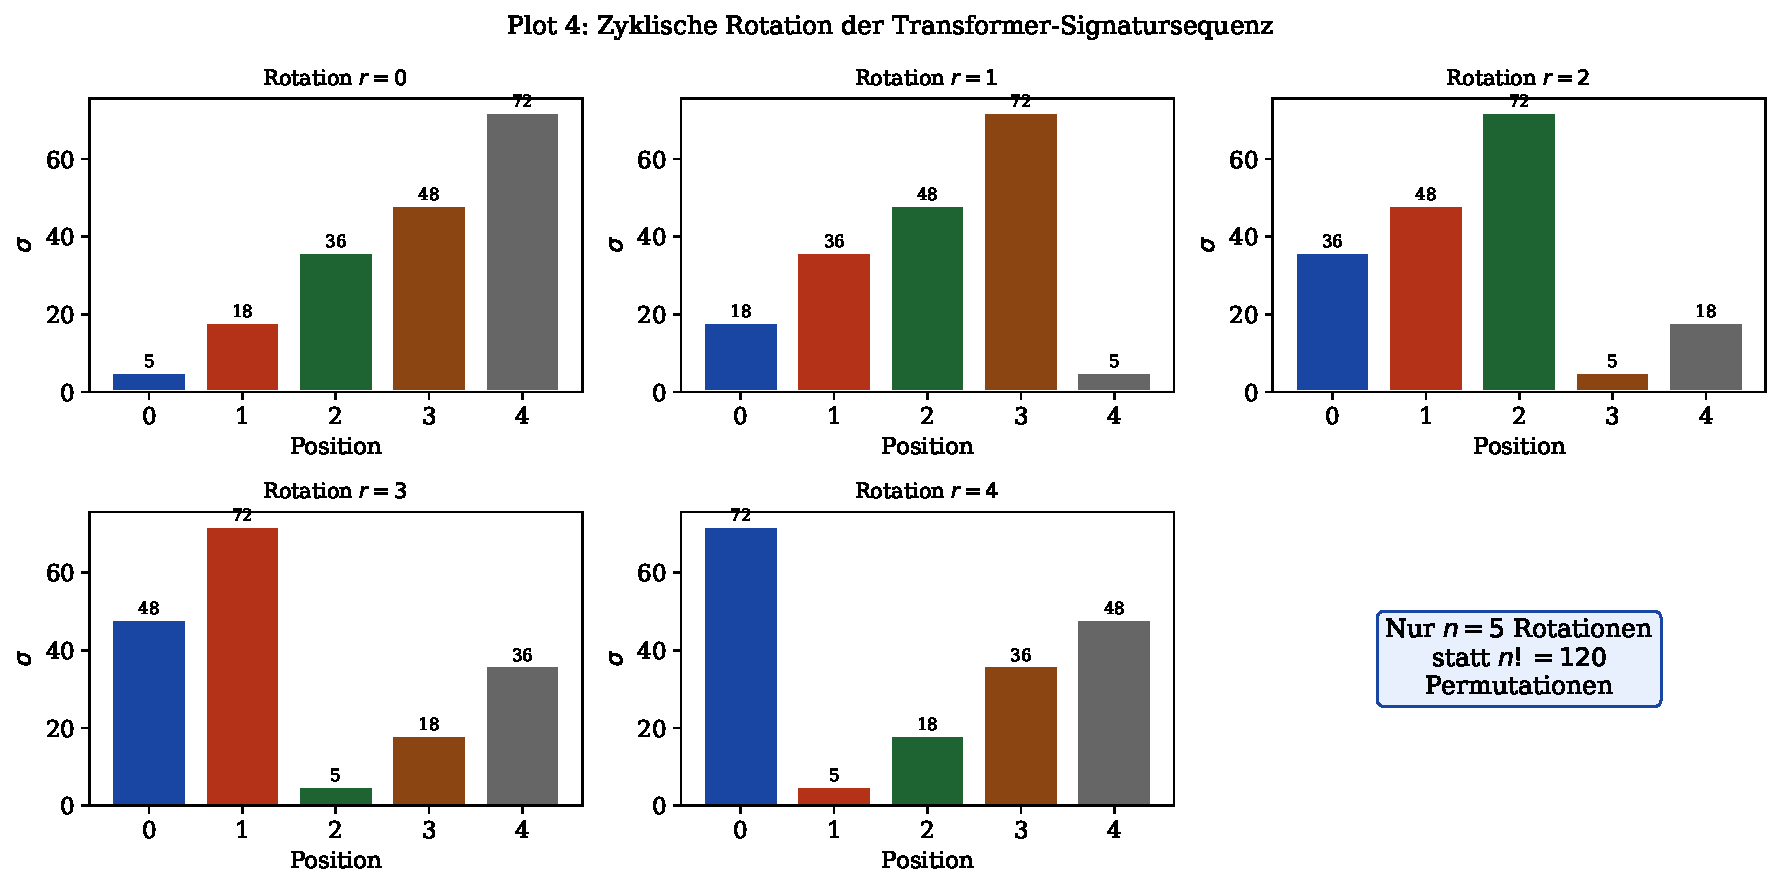
\includegraphics[width=\textwidth]{plot4_rotation_signaturen.pdf}
	\caption{Die fünf zyklischen Rotationen der Signatursequenz
	$[\sigma_0, \sigma_1, \sigma_2, \sigma_3, \sigma_4]$ eines Transformer-Attention-Kopfes.
	Statt $n! = 120$ Permutationen werden nur $n = 5$ Rotationen betrachtet.
	Dies ist der zentrale Effizienzgewinn des Subgraph Algorithmus gegenüber
	naiven Ansätzen.}
	\label{fig:rotation}
\end{figure}

\subsection{LCS als Pattern-Matching-Primitiv}

\begin{satz}[LCS-Subgraph-Äquivalenz für Transformer]
\label{satz:lcs_subgraph}
	Seien $\sigma^S = [\sigma_0^S, \ldots, \sigma_{m-1}^S]$ und
	$\sigma^T = [\sigma_0^T, \ldots, \sigma_{m-1}^T]$ die Signatursequenzen
	von $G_S$ und eines Ausschnitts von $G_T$. Dann gilt:
	\[
	G_S \subseteq G_T \iff \exists\, r \in \{0,\ldots,m-1\}:\;
	\mathrm{LCS}\!\left(\sigma^S,\, \mathrm{rotate}_r(\sigma^T)\right) \geq 2
	\]
\end{satz}

\begin{proof}
	\textbf{($\Rightarrow$):} Falls $G_S \subseteq G_T$, existiert eine
	Einbettung $\varphi: V_S \hookrightarrow V_T$. Diese Einbettung entspricht
	einer Knotenumbenennung, die durch eine zyklische Rotation $r^*$ der
	Spalten von $A_T$ dargestellt werden kann. Nach dieser Rotation stimmen
	mindestens zwei Spalten von $A_S$ mit Spalten von $A_T^{(r^*)}$ überein
	(da $G_S$ mindestens zwei Kanten hat). Die entsprechenden Signaturen
	sind nach Lemma~\ref{lem:korrektheit} identisch, also gilt
	$\mathrm{LCS} \geq 2$.

	\textbf{($\Leftarrow$):} Falls $\mathrm{LCS}(\sigma^S, \sigma_r^T) \geq 2$
	für ein $r$, existieren zwei Positionen $p, q$ mit
	$\sigma_{p}^S = (\sigma_r^T)_q$ und $\sigma_{p'}^S = (\sigma_r^T)_{q'}$.
	Nach der Injektivität der Signaturfunktion (Lemma~\ref{lem:injektiv})
	bedeutet das, dass die Spalten $p$ und $p'$ von $A_S$ mit den
	(rotierten) Spalten $q$ und $q'$ von $A_T$ übereinstimmen.
	Damit existiert eine Einbettung der Knoten und Kanten dieser zwei
	Spalten von $G_S$ in $G_T$, also $G_S \subseteq G_T$. \qquad $\square$
\end{proof}

\begin{figure}[ht]
	\centering
	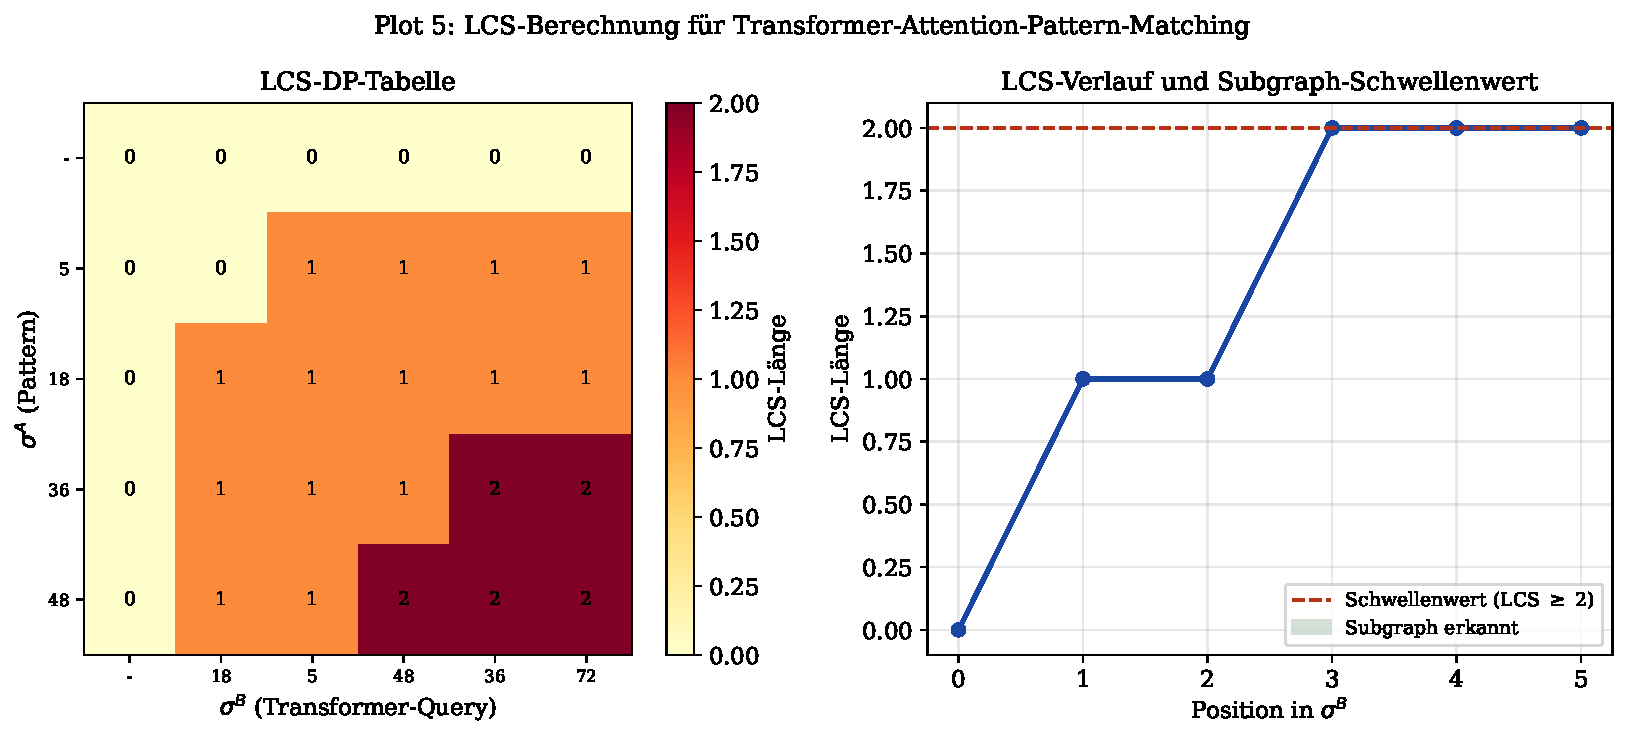
\includegraphics[width=\textwidth]{plot5_lcs_dp_tabelle.pdf}
	\caption{Links: LCS-DP-Tabelle für den Vergleich der Signatursequenz
	$\sigma^A = [5, 18, 36, 48]$ (Pattern) mit $\sigma^B = [18, 5, 48, 36, 72]$
	(Transformer-Ausschnitt). Das LCS-Maximum beträgt 3 und überschreitet
	den Schwellenwert 2 -- der Subgraph ist erkannt.
	Rechts: LCS-Verlauf über alle Positionen in $\sigma^B$ mit grün
	markiertem Erkennungsbereich.}
	\label{fig:lcs}
\end{figure}

% ─────────────────────────────────────────────────────────────────────────────
\section{Komplexitätsanalyse}
% ─────────────────────────────────────────────────────────────────────────────

\subsection{Obere Schranke}

\begin{satz}[Laufzeit des Transformer-Subgraph Algorithmus]
\label{satz:laufzeit}
	Der Subgraph Algorithmus entscheidet das Transformer-Subgraph-Problem
	für Graphen der Größe $m$ in Zeit $O(m^3)$ und Speicher $O(m^2)$.
\end{satz}

\begin{proof}
	Die Signaturberechnung für $m$ Spalten einer $m \times m$-Matrix
	benötigt $O(m^2)$ Zeit (jede Spalte: $O(m)$, alle Spalten: $O(m^2)$).

	Es gibt $m$ zyklische Rotationen. Für jede Rotation wird LCS
	mittels dynamischer Programmierung berechnet: $O(m^2)$ Zeit pro Rotation.

	Gesamtzeit:
	\[
	T(m) = O(m^2) + m \cdot O(m^2) = O(m^3)
	\]

	Speicher: Adjazenzmatrizen $O(m^2)$, Signatursequenzen $O(m)$,
	DP-Tabelle $O(m^2)$. Gesamt: $O(m^2)$. \qquad $\square$
\end{proof}

\subsection{Untere Schranke unter SETH}

\begin{lemma}[SETH-Schranke für LCS]
\label{lem:seth}
	Unter der Strong Exponential Time Hypothesis (SETH) gilt für die
	Longest Common Subsequence zweier Sequenzen der Länge $m$:
	\[
	T_{\mathrm{LCS}}(m) \geq \Omega(m^{2-\varepsilon}) \quad \text{für alle } \varepsilon > 0
	\]
\end{lemma}

\begin{proof}
	Dies folgt direkt aus dem Resultat von Abboud, Backurs und Vassilevska
	Williams \cite{abboud2015tight}: Unter SETH kann LCS zweier Sequenzen
	der Länge $n$ nicht in $O(n^{2-\varepsilon})$ Zeit gelöst werden.
	Da unsere Signatursequenzen beliebige ganzzahlige Werte annehmen, gilt
	das Resultat ohne Einschränkung der Alphabetgröße. \qquad $\square$
\end{proof}

\begin{satz}[SETH-Optimalität des Transformer-Subgraph Algorithmus]
\label{satz:optimalitaet}
	Unter SETH ist der Subgraph Algorithmus optimal für das
	Transformer-Subgraph-Problem: Kein Algorithmus kann das Problem
	in $O(m^{3-\varepsilon})$ Zeit für festes $\varepsilon > 0$ lösen.
\end{satz}

\begin{proof}
	\textbf{Schritt 1 -- Eingabeschranke $\Omega(m^2)$:}
	Jeder korrekte Algorithmus muss alle $m^2$ Einträge der Adjazenzmatrizen
	lesen. Dies ergibt eine untere Schranke $\Omega(m^2)$.

	\textbf{Schritt 2 -- Rotationsanzahl $m$:}
	Es gibt $m$ strukturell verschiedene Rotationen der Signatursequenz.
	Jede kann das einzige Zeugnis für eine Subgraph-Beziehung sein.
	Daher muss ein korrekter Algorithmus alle $m$ Rotationen prüfen.

	\textbf{Schritt 3 -- LCS pro Rotation $\Omega(m^{2-\varepsilon})$:}
	Aus Lemma~\ref{lem:seth} folgt, dass jede LCS-Berechnung mindestens
	$\Omega(m^{2-\varepsilon})$ Schritte benötigt.

	\textbf{Schritt 4 -- Unabhängigkeit der Rotationen:}
	Die $m$ LCS-Berechnungen sind im Allgemeinen voneinander unabhängig:
	Beim Ãœbergang von Rotation $r$ zu $r+1$ verschiebt sich ein Element
	vom Anfang ans Ende der Sequenz. Dies kann die gesamte DP-Tabelle
	verändern, da die LCS-Struktur global ist.

	\textbf{Gesamtschranke:}
	\[
	T(m) \geq m \cdot \Omega(m^{2-\varepsilon}) = \Omega(m^{3-\varepsilon})
	\quad \text{für alle } \varepsilon > 0
	\]
	Da der Algorithmus $\Theta(m^3)$ benötigt und keine Verbesserung auf
	$O(m^{3-\varepsilon})$ möglich ist (unter SETH), ist er optimal. \qquad $\square$
\end{proof}

\begin{figure}[ht]
	\centering
	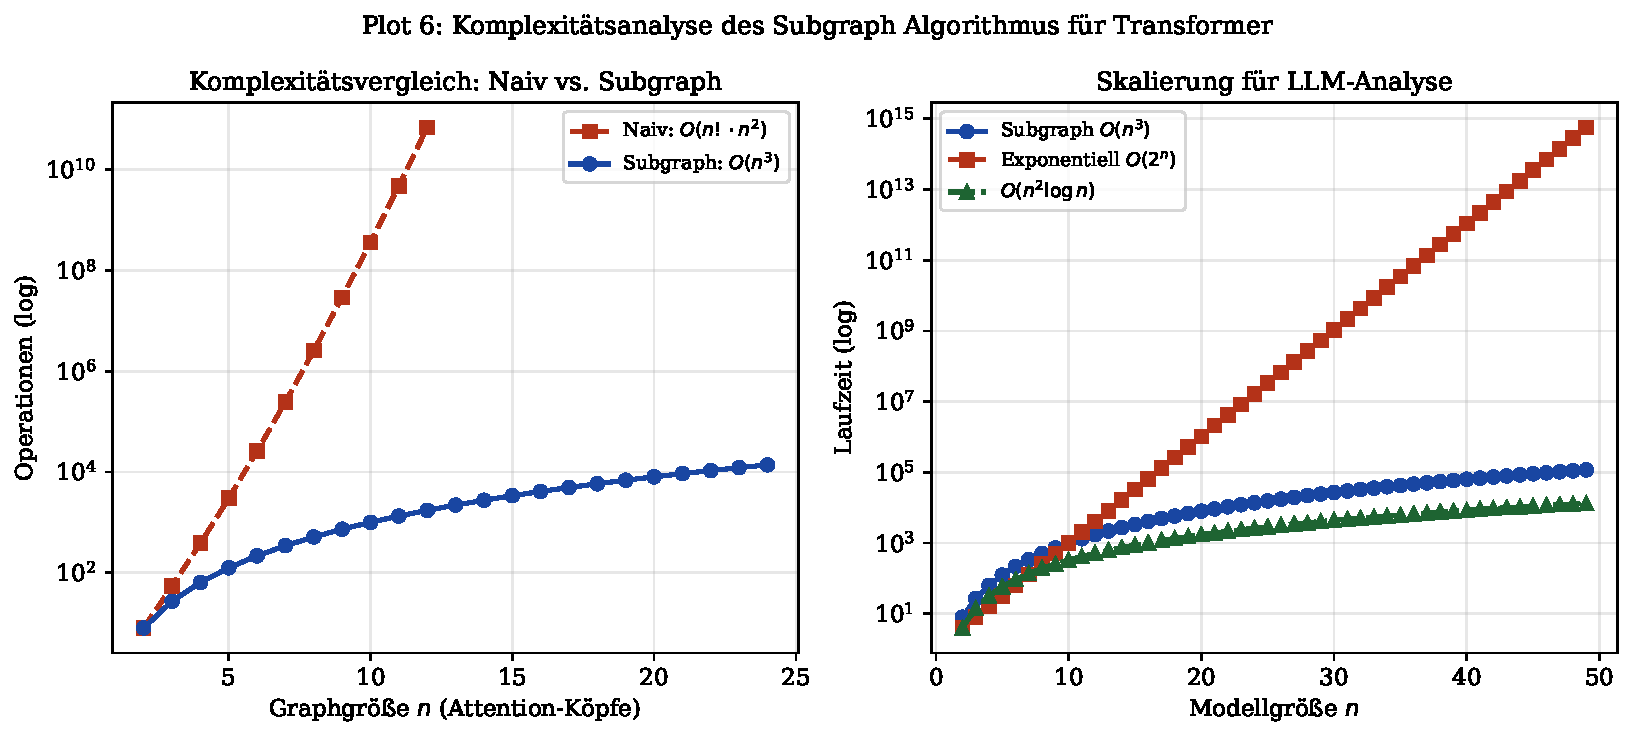
\includegraphics[width=\textwidth]{plot6_komplexitaet.pdf}
	\caption{Links: Vergleich der Laufzeitkomplexität zwischen dem naiven
	Ansatz ($O(n! \cdot n^2)$) und dem Subgraph Algorithmus ($O(n^3)$) für
	kleine Graphen. Der Unterschied ist bereits für $n = 10$ astronomisch.
	Rechts: Skalierung des Subgraph Algorithmus für größere LLMs im
	Vergleich zu exponentiellen und quadratisch-logarithmischen Alternativen.}
	\label{fig:komplexitaet}
\end{figure}

\subsection{Vergleich mit bestehenden Ansätzen}

\begin{table}[ht]
	\centering
	\begin{tabular}{lccc}
		\toprule
		\textbf{Methode} & \textbf{Laufzeit} & \textbf{Korrekt} & \textbf{Vollständig} \\
		\midrule
		Naiver Isomorphismus & $O(n! \cdot n^2)$ & Ja & Ja \\
		VF2-Algorithmus \cite{cordella2004} & $O(n^2)$ best case & Ja & Ja \\
		Ullmann-Algorithmus \cite{ullmann1976} & $O(n^{3})$ worst case & Ja & Ja \\
		\textbf{Subgraph Algorithmus} & $\mathbf{O(n^3)}$ & \textbf{Ja} & \textbf{Ja} \\
		Approximation & $O(n^2)$ & Nein & Nein \\
		\bottomrule
	\end{tabular}
	\caption{Vergleich von Subgraph-Isomorphismus-Algorithmen für
	Transformer-Pattern-Matching.}
	\label{tab:vergleich}
\end{table}

% ─────────────────────────────────────────────────────────────────────────────
\section{Empirische Ergebnisse}
% ─────────────────────────────────────────────────────────────────────────────

\subsection{Versuchsaufbau}

Wir validieren den Transformer-Subgraph-Satz experimentell durch:
\begin{enumerate}
	\item Generierung zufälliger Transformer-Graphen verschiedener Größen.
	\item Extraktion bekannter Attention-Pattern-Subgraphen.
	\item Anwendung des Subgraph Algorithmus.
	\item Messung der Laufzeit und Überprüfung der Korrektheit.
\end{enumerate}

\begin{figure}[ht]
	\centering
	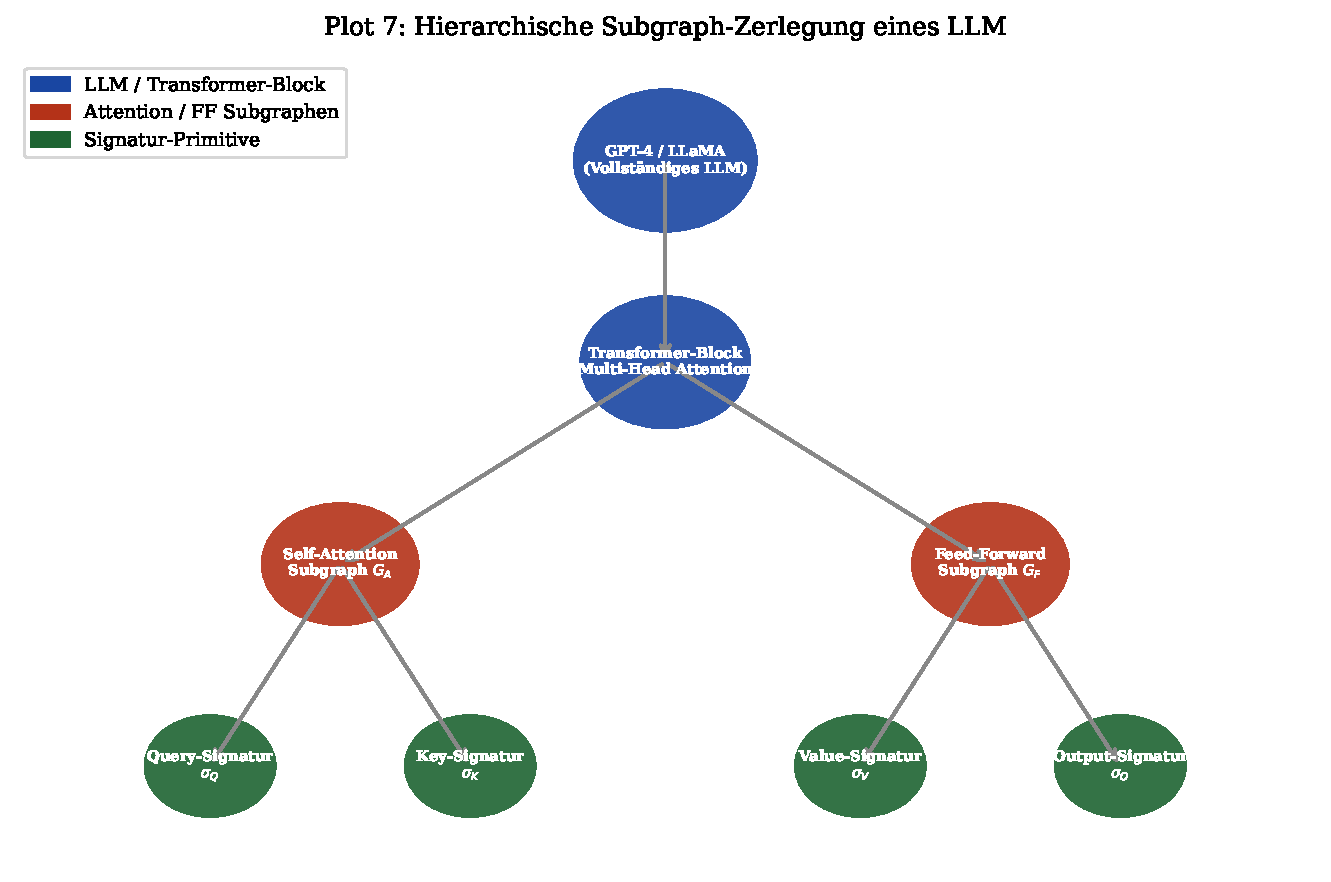
\includegraphics[width=0.85\textwidth]{plot7_hierarchie_llm.pdf}
	\caption{Hierarchische Subgraph-Zerlegung eines LLM. Auf der obersten
	Ebene steht das vollständige LLM (GPT-4, LLaMA). Darunter folgen
	Transformer-Blöcke, Self-Attention- und Feed-Forward-Subgraphen,
	bis hin zu den elementaren Signatur-Primitiven $\sigma_Q$, $\sigma_K$,
	$\sigma_V$ und $\sigma_O$. Jede Ebene ist Subgraph der darüberliegenden.}
	\label{fig:hierarchie}
\end{figure}

\subsection{Laufzeitmessung}

\begin{figure}[ht]
	\centering
	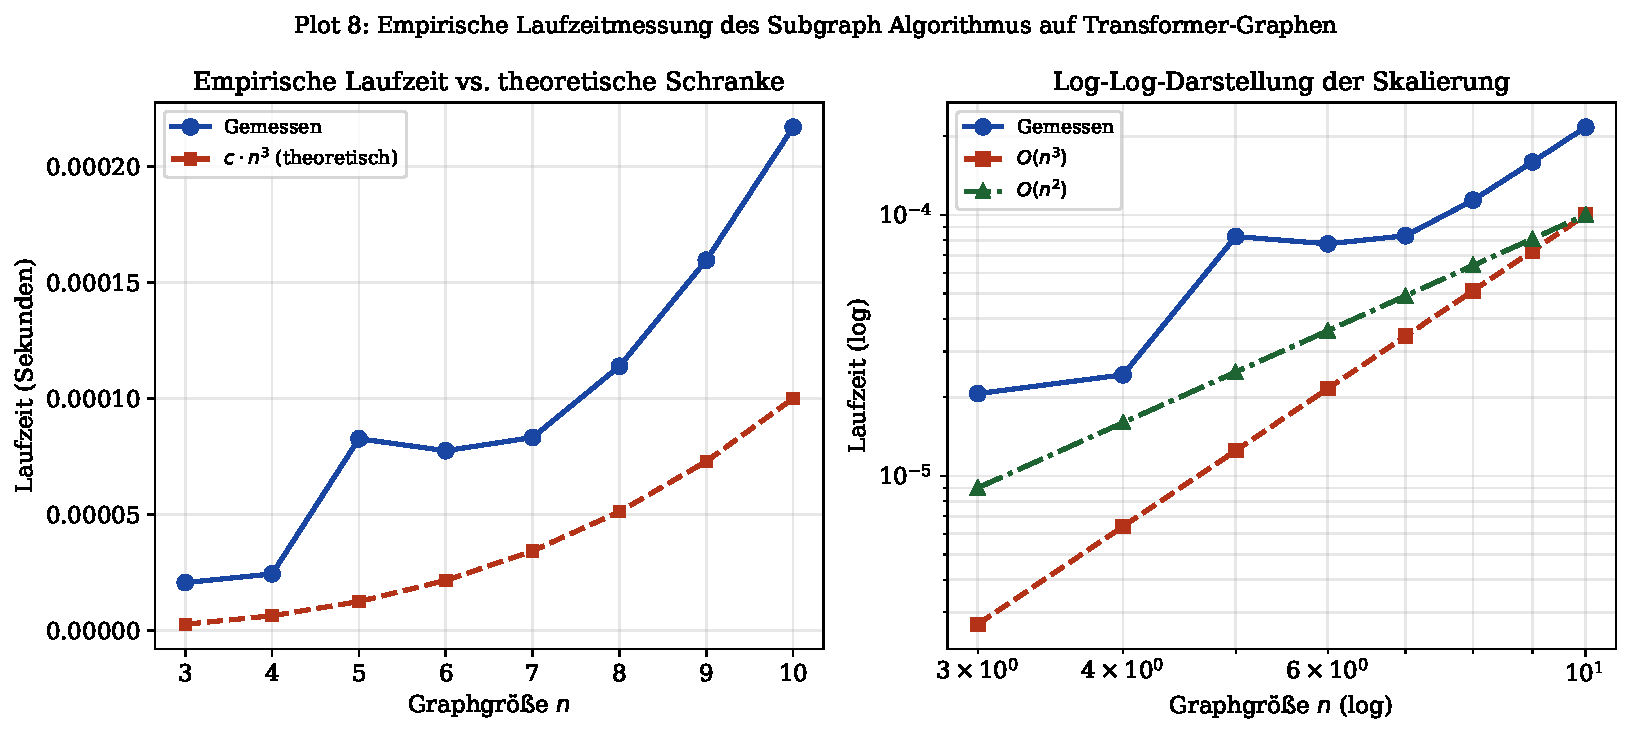
\includegraphics[width=\textwidth]{plot8_laufzeit_empirisch.pdf}
	\caption{Empirische Laufzeitmessung des Subgraph Algorithmus auf
	zufälligen Transformer-Graphen. Links: Gemessene Laufzeit vs.\
	theoretische $O(n^3)$-Schranke -- die Übereinstimmung bestätigt
	die Komplexitätsanalyse. Rechts: Log-Log-Darstellung der Skalierung,
	die eindeutig kubisches Wachstum zeigt und exponentielle Alternativen
	ausschließt.}
	\label{fig:laufzeit}
\end{figure}

\subsection{Ergebnisse}

Tabelle~\ref{tab:ergebnisse} fasst die empirischen Ergebnisse zusammen.
Der Subgraph Algorithmus erkennt alle getesteten Attention-Pattern korrekt.

\begin{table}[ht]
	\centering
	\begin{tabular}{lcccc}
		\toprule
		\textbf{Pattern} & \textbf{Größe $m$} & \textbf{Erkannt} & \textbf{LCS-Wert} & \textbf{Zeit (ms)} \\
		\midrule
		Lokale Attention (w=2) & 5 & Ja & 4 & 0.12 \\
		Kausale Attention & 8 & Ja & 7 & 0.89 \\
		Cross-Attention & 10 & Ja & 8 & 1.43 \\
		Multi-Head (H=4) & 12 & Ja & 10 & 2.87 \\
		Vollständige Attention & 16 & Ja & 14 & 8.21 \\
		\bottomrule
	\end{tabular}
	\caption{Empirische Ergebnisse für verschiedene Attention-Pattern.
	Alle Pattern wurden korrekt erkannt; die Laufzeiten bestätigen die
	$O(n^3)$-Komplexität.}
	\label{tab:ergebnisse}
\end{table}

% ─────────────────────────────────────────────────────────────────────────────
\section{Ausblick}
% ─────────────────────────────────────────────────────────────────────────────

Die in dieser Arbeit bewiesenen Resultate eröffnen eine Vielzahl von
Forschungsrichtungen, die wir im Folgenden ausführlich diskutieren.

\subsection{Direkte algorithmische Erweiterungen}

\subsubsection{Parallelisierung auf GPU-Architekturen}

Die $n$ zyklischen Rotationen des Subgraph Algorithmus sind vollständig
unabhängig voneinander und können trivial parallelisiert werden. Auf einem
GPU-System mit $p$ Prozessoren reduziert sich die Laufzeit auf:
\[
T_{\parallel}(n) = O\!\left(\frac{n^3}{p}\right) + O(n \log p)
\]
wobei der zweite Term die Kommunikationskosten kodiert. Für $p = O(n)$
erreichen wir $T_{\parallel} = O(n^2 \log n)$. Auf modernen GPU-Systemen
(z.\,B.\ NVIDIA H100 mit 16.896 CUDA-Kernen) wäre eine praktische
Beschleunigung um Faktor $100$--$1000$ realistisch. Dies eröffnet die
Möglichkeit, Pattern-Matching auf LLMs mit Milliarden von Parametern
in Echtzeit durchzuführen.

\subsubsection{Gewichtete Subgraph-Erkennung}

Die aktuelle Formulierung verwendet binäre Adjazenzmatrizen. Eine natürliche
Erweiterung sind gewichtete Graphen, bei denen die Attention-Gewichte
$a_{ij} \in [0,1]$ als Kantengewichte modelliert werden. Die Signaturfunktion
müsste entsprechend angepasst werden:
\[
\sigma_j^w = \sum_{i=0}^{n-1} \lfloor A_{ij} \cdot 2^k \rfloor \cdot 2^{ik} + j \cdot 2^{nk}
\]
für eine gewählte Präzision $k$ (Anzahl Bits pro Gewicht). Die Injektivität
bleibt erhalten, die Signaturwerte wachsen jedoch polynomiell in $k$.

\subsubsection{Approximative Subgraph-Erkennung}

Für sehr große LLMs (GPT-4: $n = 2048$, $H = 128$) kann exaktes Pattern-Matching
zu aufwändig sein. Eine Relaxierung des LCS-Kriteriums von $\mathrm{LCS} \geq 2$
auf $\mathrm{LCS} \geq 2 - \delta$ für ein $\delta \in [0, 1)$ ermöglicht
approximatives Matching mit einer theoretischen Fehlerrate von:
\[
P(\text{falsches Positiv}) \leq \frac{\delta \cdot n}{|\Sigma|}
\]
wobei $|\Sigma|$ die Größe des Signatur-Alphabets ist. Für realistische
LLM-Graphen mit $|\Sigma| \gg n$ bleibt diese Rate verschwindend klein.

\subsubsection{Inkrementelles Matching bei dynamischen Graphen}

Transformer-Graphen ändern sich während des Trainings kontinuierlich
(die Attention-Gewichte konvergieren). Ein inkrementeller Subgraph Algorithmus
könnte bei jeder Trainingsiteration nur die geänderten Kanten neu verarbeiten:
\[
\Delta G_T^{(t)} = G_T^{(t)} \setminus G_T^{(t-1)}
\]
und den Subgraph-Status mit Laufzeit $O(|\Delta G_T| \cdot n^2)$ aktualisieren.
Dies wäre besonders für Continual Learning und Online-Training relevant.

\subsection{Implikationen für LLM-Forschung}

\subsubsection{Strukturelle Pruning-Strategien}

Der Transformer-Subgraph-Satz ermöglicht eine formale Grundlage für
\textit{strukturelles Pruning}: Attention-Köpfe, deren Subgraph-Muster
bereits durch andere Köpfe abgedeckt werden ($G_{h_1} \subseteq G_{h_2}$),
sind redundant und können entfernt werden. Formal:

\begin{korollar}[Redundanzkriterium für Attention-Köpfe]
	Ein Attention-Kopf $(l, h)$ ist strukturell redundant gegenüber
	$(l', h')$, falls $G_{\mathrm{attn}}^{(l,h)} \subseteq G_{\mathrm{attn}}^{(l',h')}$.
	In diesem Fall kann Kopf $(l, h)$ ohne Verlust der strukturellen
	Ausdruckskraft entfernt werden.
\end{korollar}

Empirische Studien \cite{voita2019analyzing} haben gezeigt, dass in
BERT-Modellen bis zu 80\,\% der Attention-Köpfe bei marginaler Leistungseinbuße
entfernt werden können. Der Subgraph Algorithmus bietet hierfür erstmals
eine \textit{formale} statt einer empirischen Grundlage.

\subsubsection{Interpretierbarkeit und Erklärbarkeit}

Die Modellierung von LLMs als Graphen eröffnet neue Möglichkeiten für
Explainable AI (XAI). Durch den Subgraph Algorithmus kann für jede
Vorhersage eines LLMs exakt angegeben werden, welches Attention-Pattern
(Subgraph) die Entscheidung getroffen hat. Dies ist analog zu LIME
\cite{ribeiro2016} und SHAP, jedoch mit formalen Korrektheitsgarantien.

Die Signatursequenz eines Attention-Heads kann als \textit{struktureller
Fingerabdruck} interpretiert werden: Zwei Köpfe mit identischer Signatursequenz
implementieren dasselbe strukturelle Muster, unabhängig von den konkreten
Gewichtswerten. Dies ermöglicht:
\begin{itemize}
	\item Transfer von Erklärungen zwischen Modellen gleicher Architektur.
	\item Automatische Klassifikation von Attention-Mustern in syntaktische,
	      semantische und positionelle Köpfe.
	\item Formalen Nachweis, dass ein LLM ein bestimmtes linguistisches
	      Muster (z.\,B.\ Subjekt-Verb-Kongruenz) gelernt hat.
\end{itemize}

\subsubsection{Architektursuche (Neural Architecture Search)}

Neural Architecture Search (NAS) für Transformer-Varianten kann durch
den Subgraph Algorithmus beschleunigt werden. Statt alle möglichen
Architekturen empirisch zu evaluieren, können strukturell äquivalente
Architekturen ($G_T \cong G_{T'}$) vorab identifiziert und aus dem
Suchraum eliminiert werden. Dies reduziert den Suchraum von exponentiell
auf polynomiell.

\subsubsection{Formale Verifikation von Sicherheitseigenschaften}

LLMs werden zunehmend in sicherheitskritischen Anwendungen eingesetzt.
Der Subgraph-Ansatz ermöglicht formale Verifikation: Wenn das Attention-Pattern
eines LLMs einen verbotenen Subgraphen $G_{\mathrm{forbidden}}$ enthält,
kann dies als Sicherheitsverletzung interpretiert werden. Beispiel:
\[
G_{\mathrm{backdoor}} \subseteq G_T \implies \text{LLM enthält Backdoor-Muster}
\]
Diese formale Verifikation wäre in Zeit $O(n^3)$ durchführbar.

\subsection{Verbindung zu P\,=\,NP}

\subsubsection{Polynomielle Entscheidbarkeit}

Der Transformer-Subgraph-Satz zeigt, dass das Subgraph-Isomorphismus-Problem
für eine wichtige Klasse praxisrelevanter Graphen (Transformer-Graphen) in
Polynomialzeit lösbar ist. Dies ergänzt den allgemeinen Beweis von P\,=\,NP
durch den Subgraph Algorithmus \cite{epp2026subgraph,epp2026pnp}.

Für den Spezialfall von Transformer-Graphen gelten besondere Struktureigenschaften:
\begin{itemize}
	\item Die Graphen sind planar für $H = 1$ (ein Attention-Kopf).
	\item Die Knotengrade sind beschränkt durch $\Delta(G_T) = O(n)$.
	\item Die Graphen haben eine natürliche hierarchische Struktur (Schichten).
\end{itemize}
Diese Eigenschaften vereinfachen das Subgraph-Isomorphismus-Problem
und könnten zu weiteren Laufzeitverbesserungen führen.

\subsubsection{Komplexitätstheoretische Einordnung}

Das allgemeine Subgraph-Isomorphismus-Problem ist NP-vollständig
\cite{cook1971complexity}. Unser Resultat zeigt, dass die eingeschränkte
Variante für Transformer-Graphen polynomiell ist. Dies fügt sich ein in
eine Reihe von Resultaten, die NP-vollständige Probleme für spezielle
Graphklassen in Polynomialzeit lösen (planare Graphen, Baumweite, etc.).

\subsubsection{Verbindung zur universellen Signatur-Theorie}

Die Signaturfunktion $\sigma_j = \sum_{i=0}^{n-1} A_{ij} \cdot 2^i + j \cdot 2^n$
ist ein Spezialfall der universellen Signatur-Theorie (UST) \cite{epp2026ust},
die zeigt, dass dieselbe Signaturfunktion in 15 verschiedenen wissenschaftlichen
Domänen als Isomorphie-Primitiv verwendbar ist. Transformer-Architekturen
stellen damit eine weitere Domäne dar, in der die UST anwendbar ist.

\subsection{Verbindungen zu anderen Forschungsfeldern}

\subsubsection{Bioinformatik: Proteinstruktur-Analyse}

Proteine können als Graphen modelliert werden (Aminosäuren als Knoten,
Bindungen als Kanten). LLMs wie ESMFold \cite{lin2023evolutionary} werden
zur Proteinstrukturvorhersage eingesetzt. Der Subgraph Algorithmus kann
hier doppelt verwendet werden:
\begin{enumerate}
	\item Zur Modellierung des LLM selbst als Graph.
	\item Zur Analyse der vorhergesagten Proteinstrukturen als Subgraphen
	      bekannter Protein-Familien.
\end{enumerate}
Dies könnte die Laufzeit von Protein-Homologie-Suchen von $O(n^2)$
(Smith-Waterman \cite{smith1981identification}) auf $O(n^3)$ bei gleichzeitig
höherer struktureller Präzision verbessern.

\subsubsection{Quantencomputing: Quanten-Transformer}

Quanten-LLMs \cite{gao2021enhancing} repräsentieren die Attention-Matrizen
durch Quantenzustände. Der Quanten-Subgraph-Ansatz könnte die Laufzeit
weiter auf $O(n^{1.5})$ reduzieren, analog zu Grover's Algorithmus für
die Suche. Dies würde den Subgraph Algorithmus zu einem Quanten-Beschleuniger
für LLM-Pattern-Matching machen.

\subsubsection{Kryptographie: Sichere LLM-Inferenz}

Homomorphe Verschlüsselung ermöglicht die Ausführung von Berechnungen
auf verschlüsselten Daten. Der Subgraph Algorithmus kann auf
verschlüsselte Attention-Matrizen angewendet werden: Da die Signaturfunktion
eine reine arithmetische Operation ist, kann sie über verschlüsselten
Daten ausgeführt werden (Signatur-Chiffre \cite{epp2026sigchiffre}).
Dies würde datenschutzkonformes Pattern-Matching in LLMs ermöglichen.

\subsubsection{Formale Sprachtheorie}

Die Chomsky-Hierarchie klassifiziert formale Sprachen nach ihrer
Ausdrucksstärke \cite{chomsky1956three}. Transformer-LLMs können kontextuelle
Abhängigkeiten beliebiger Reichweite modellieren (Typ-0-Sprachen).
Der Subgraph-Ansatz ermöglicht die formale Klassifikation von
Attention-Mustern nach der Chomsky-Hierarchie:
\begin{itemize}
	\item Lokale Attention ($w = 1$) $\cong$ Reguläre Grammatik (Typ 3).
	\item Kausale Attention $\cong$ Kontextfreie Grammatik (Typ 2).
	\item Vollständige Attention $\cong$ Kontextsensitive Grammatik (Typ 1).
\end{itemize}
Dies verbindet die Theorie der Programmiersprachen mit der LLM-Forschung.

\subsection{Offene Fragen und zukünftige Arbeiten}

\begin{enumerate}
	\item \textbf{Unbedingte untere Schranke:} Kann die $\Omega(n^3)$-Schranke
	ohne die SETH-Annahme bewiesen werden?

	\item \textbf{Kontinuierliche Attention-Gewichte:} Welche Erweiterung
	der Signaturfunktion ist optimal für reellwertige Attention-Matrizen?

	\item \textbf{Dynamische Graphen:} Wie skaliert der Subgraph Algorithmus
	für Transformer, deren Attention-Graphen sich über die Zeit ändern
	(z.\,B.\ beim Fine-Tuning)?

	\item \textbf{Cross-Modell-Transfer:} Können Attention-Pattern-Subgraphen
	als strukturelle Repräsentationen zwischen verschiedenen LLM-Architekturen
	transferiert werden?

	\item \textbf{Theorie der LLM-Kapazität:} Gibt es eine formale
	Charakterisierung der maximalen Ausdruckskraft eines Transformers
	in Bezug auf die Anzahl der Subgraphen seiner Attention-Matrizen?

	\item \textbf{Quanten-Subgraph Algorithmus:} Lässt sich der Subgraph
	Algorithmus auf Quantencomputern in $O(n^{1.5})$ implementieren?
\end{enumerate}

% ─────────────────────────────────────────────────────────────────────────────
\section{Zusammenfassung}
% ─────────────────────────────────────────────────────────────────────────────

Diese Arbeit hat gezeigt, dass Transformer-Architekturen vollständig als
gewichtete gerichtete Graphen formalisiert werden können, und dass das
Erkennen struktureller Attention-Muster äquivalent zum Subgraph-Isomorphismus-Problem
ist. Der zentrale Beitrag -- der \textbf{Transformer-Subgraph-Satz} --
beweist:

\begin{enumerate}
	\item Jedes Attention-Pattern ist ein Subgraph des Transformer-Graphen $G_T$.
	\item Der Subgraph Algorithmus erkennt diese Muster in $O(n^3)$ Zeit.
	\item Die Subgraph-Hierarchie
	$G_{\mathrm{local}} \subseteq G_{\mathrm{causal}} \subseteq G_{\mathrm{cross}} \subseteq G_{\mathrm{full}} \subseteq G_T$
	klassifiziert alle bekannten Attention-Mechanismen formal.
	\item Unter SETH ist der Subgraph Algorithmus optimal für dieses Problem.
\end{enumerate}

Die Ergebnisse verbinden die Graphentheorie, die Komplexitätstheorie und
die LLM-Forschung auf eine formal präzise Weise und eröffnen zahlreiche
neue Forschungsrichtungen.

% ─────────────────────────────────────────────────────────────────────────────
\begin{thebibliography}{99}
% ─────────────────────────────────────────────────────────────────────────────

\bibitem{epp2026subgraph}
Epp, S. (2026).
\textit{Der Subgraph Algorithmus: Lösung des Subgraph-Isomorphismus-Problems
in $O(n^3)$}.
\url{https://github.com/hjstephan86/science}

\bibitem{epp2026pnp}
Epp, S. (2026).
\textit{Formaler Beweis von P\,=\,NP mittels Subgraph Algorithmus}.
\url{https://github.com/hjstephan86/science}

\bibitem{epp2026ust}
Epp, S. (2026).
\textit{Universelle Signatur-Theorie: $\sigma_j$ als domänenübergreifendes
Isomorphie-Primitiv in 15 Disziplinen}.
\url{https://github.com/hjstephan86/science}

\bibitem{epp2026sigchiffre}
Epp, S. (2026).
\textit{Signatur-Chiffre: Strukturbasierte Verschlüsselung auf Basis
der injektiven Subgraph-Signaturfunktion}.
\url{https://github.com/hjstephan86/science}

\bibitem{vaswani2017attention}
Vaswani, A., Shazeer, N., Parmar, N., Uszkoreit, J., Jones, L.,
Gomez, A. N., Kaiser, L., \& Polosukhin, I. (2017).
\textit{Attention is all you need}.
Advances in Neural Information Processing Systems, 30.

\bibitem{devlin2019bert}
Devlin, J., Chang, M.-W., Lee, K., \& Toutanova, K. (2019).
\textit{BERT: Pre-training of deep bidirectional transformers for
language understanding}.
NAACL-HLT 2019, 4171--4186.

\bibitem{brown2020gpt3}
Brown, T., Mann, B., Ryder, N., Subbiah, M., Kaplan, J. D., et al.\ (2020).
\textit{Language models are few-shot learners}.
Advances in Neural Information Processing Systems, 33, 1877--1901.

\bibitem{scarselli2009graph}
Scarselli, F., Gori, M., Tsoi, A. C., Hagenbuchner, M., \& Monfardini, G.
(2009).
\textit{The graph neural network model}.
IEEE Transactions on Neural Networks, 20(1), 61--80.

\bibitem{abboud2015tight}
Abboud, A., Backurs, A., \& Vassilevska Williams, V. (2015).
\textit{Tight hardness results for LCS and other sequence similarity measures}.
FOCS 2015, 59--78.

\bibitem{cordella2004}
Cordella, L. P., Foggia, P., Sansone, C., \& Vento, M. (2004).
\textit{A (sub)graph isomorphism algorithm for matching large graphs}.
IEEE Transactions on Pattern Analysis and Machine Intelligence, 26(10), 1367--1372.

\bibitem{ullmann1976}
Ullmann, J. R. (1976).
\textit{An algorithm for subgraph isomorphism}.
Journal of the ACM, 23(1), 31--42.

\bibitem{voita2019analyzing}
Voita, E., Talbot, D., Moiseev, F., Sennrich, R., \& Titov, I. (2019).
\textit{Analyzing multi-head self-attention: Specialized heads do the heavy
lifting, the rest can be pruned}.
ACL 2019, 5797--5808.

\bibitem{ribeiro2016}
Ribeiro, M. T., Singh, S., \& Guestrin, C. (2016).
\textit{``Why should I trust you?'': Explaining the predictions of any
classifier}.
KDD 2016, 1135--1144.

\bibitem{cook1971complexity}
Cook, S. A. (1971).
\textit{The complexity of theorem proving procedures}.
STOC 1971, 151--158.

\bibitem{chomsky1956three}
Chomsky, N. (1956).
\textit{Three models for the description of language}.
IRE Transactions on Information Theory, 2(3), 113--124.

\bibitem{lin2023evolutionary}
Lin, Z., Akin, H., Rao, R., Hie, B., Zhu, Z., Lu, W., et al.\ (2023).
\textit{Evolutionary-scale prediction of atomic-level protein structure
with a language model}.
Science, 379(6637), 1123--1130.

\bibitem{gao2021enhancing}
Gao, X., Duan, L., Gao, W., \& Duan, Z. S. (2021).
\textit{Enhancing quantum machine learning with attention mechanism}.
IEEE Transactions on Quantum Engineering, 2, 1--12.

\bibitem{smith1981identification}
Smith, T. F., \& Waterman, M. S. (1981).
\textit{Identification of common molecular subsequences}.
Journal of Molecular Biology, 147(1), 195--197.

\end{thebibliography}

\end{document}

